\section{Categorization of Errors in Transformation Networks}

%\todoLater{Discuss problem of default values, or more general \enquote{special cases}?}

\mnote{Categorization of errors}
In this section, we identify and categorize potential \emph{failures} that can occur when executing transformation networks, which are derived from the failure cases of the application algorithm discussed in \autoref{chap:orchestration}.
We consider the \emph{mistakes} and the resulting \emph{faults} in the transformation specifications, which a transformation developer can make.
The mistakes are specific for the introduced knowledge levels, thus we derive them from those levels.
We finally relate mistakes to the failures that can occur when transformation networks containing faults caused by those mistakes are still executed.


\subsection{Mistakes, Faults and Failures}

\mnote{Distinction of error types}
Errors in transformation networks can occur in different contexts, for example in terms of the transformation networks, more precisely the application algorithm, producing an incorrect result, or in terms of a transformation developer defining an erroneous transformation.
To be able to distinguish these contexts, we have already used the terms \emph{mistakes}, \emph{fault} and \emph{failure} with a short introduction of their distinction, as specializations of the general term \emph{error}.
They are supposed to describe erroneous or inappropriate knowledge of a developer (mistakes), erroneous implementations (faults) and erroneous execution results (failures).
These different types of errors depend on each other, as a mistake can lead to a fault, which can then lead to a failure.

\begin{properdescription}
    \item[Mistake:] \mnote{Erroneous knowledge}
    A mistake is made by a transformation developer. It is based on missing or erroneous knowledge about either the actual transformation or the necessity to ensure certain properties. For example, the missing knowledge that transformations must be synchronizing leads to a mistake in the conceptualization of transformations, as they do not ensure this required property. The missing knowledge that compatibility is required as well as the missing knowledge about the other transformations of a network can lead to the mistake that incompatible transformations are realized.
    If a transformation language abstracts from a conceptual level and relieves the developer from ensuring that no mistakes at that level are made, such mistakes can also be made by the transformation language developer and then manifest in a faulty implementation of the language. We do, however, not consider that case explicitly. 
    \item[Fault:] \mnote{Erroneous implementation}
    A fault is the manifestation of a mistake in the implementation of transformations. For example, the missing knowledge about the necessity to have synchronizing transformations can lead to the fault that the implementation does not properly identify existing elements instead of creating new ones. A fault is, thus, always the consequence of a mistake. It is also made by a transformation developer but can be seen within the implementation explicitly, whereas a mistake can only be detected by the fault in the implementation to which it led.
    \item[Failure:] \mnote{Manifestation of fault during execution}
    A failure occurs at execution time of transformations and is the manifestation of a fault when executing a faulty transformation network. A failure is the incorrect result of the execution of transformations. Whenever the transformations in a network have a faulty implementation, failures such as the termination in inconsistent states or non-termination of the application algorithm can occur. Since the occurrence of a failure depends on the scenario in which the transformations are executed, not every fault leads to a failure. On the other hand, a fault can also lead to several failures, e.g., because a transformation is executed multiple times.
\end{properdescription}

\mnote{Relation to other error notions}
Several similar terms like errors, mistakes, faults, bugs, defects, and so on are used in software engineering and especially in software testing.
They are sometimes used interchangeably and sometimes with specific meanings.
One common notion is the distinction of faults, errors, and failures in software testing, however also with different meanings, of which at least one is comparable to ours using the term \emph{error} for what we call \emph{mistake}.
We decided to avoid the overloaded term \emph{error} and make the human \emph{mistake} explicit.


\subsection{Possible Failure Types}
\label{chap:errors:categorization:failures}

\mnote{Essential failure types}
Failures are the manifestation of faults during transformation execution and thus the final result of mistakes made by a transformation developer.
A failure means that the execution of the transformation network, or more precisely the application algorithm, reached an unwanted state.
We have already discussed in \autoref{chap:orchestration:decidability:correctness_termination} that the application algorithm can fail by not implementing a correct application function, thus either returning models that are inconsistent or not terminating at all.
Additionally, the algorithm may fail to deliver consistent models and return $\bot$ instead.
Returning $\bot$ is actually desired behavior to deal with the undecidability of the orchestration problem.
It can, however, mask that the transformations in the network contain faults that lead to the algorithm not being able to find an orchestration that yields consistent models.

\mnote{Specialization options for failure types}
Termination in an inconsistent state, non-termination, and returning $\bot$ already form the three general failure types that can occur when executing faulty transformations.
They can be further specialized in different dimensions, e.g., regarding determinism of inconsistent termination or regarding whether too many or too few elements (or combinations of them) exist for being consistent.
The latter could manifest in missing corresponding condition elements or the existence of too many condition elements for which no consistent models can be found by adding further ones.
We have, however, found in previous work~\owncite[Tab.~5.7]{saglam2020ma} that this distinction regarding elements does not provide any insights and benefits when tracing the failures back to the causal mistakes.
We do, however, consider \emph{duplications} as one specific additional failure type, which can finally lead to any of the other failures, depending on whether the application algorithm aborts or not.
Duplications of elements are of particular importance, because they are the essential manifestation of missing synchronization in transformations, as we have discussed in \autoref{chap:synchronization:achieving}.

\begin{figure}
    \centering
    \newcommand{\labelcolumnwidth}{4.5em}
\newcommand{\contentcolumnwidth}{7em}
\newcommand{\failurecolumnfactor}{1.65}
\newcommand{\rowdistance}{6em}

\begin{tikzpicture}[
    entry/.style={font=\small}
]

    
    \node[text depth=18em, minimum width=\contentcolumnwidth+\labelcolumnwidth, minimum height=20em] %, fill=lightgray!50]
    (errors) {\textbf{Mistakes}};
    \node[right=\contentcolumnwidth+0.5*\labelcolumnwidth of errors.center, anchor=center, text depth=18em, minimum width=\contentcolumnwidth, minimum height=20em] %, fill=lightgray!25] 
    (faults) {\textbf{Faults}};
    \node[right=(0.5+0.5*\failurecolumnfactor)*\contentcolumnwidth of faults.center, anchor=center, text depth=18em, minimum width=\failurecolumnfactor*\contentcolumnwidth, minimum height=20em] %, fill=lightgray!50] 
    (failures) {\textbf{Failures}};
    
    \node[below=5em of errors.north west, anchor=west, align=left, inner sep=0.7em] (transformation) {Level 1:\\ \emph{Transfor-}\\\emph{mation}};
    \node[below=\rowdistance of transformation.west, anchor=west, align=left, inner sep=0.7em] (relation) {Level 2:\\ \emph{Network}\\\emph{Relation}};
    \node[below=\rowdistance of relation.west, anchor=west, align=left, inner sep=0.7em] (rule) {Level 3:\\ \emph{Network}\\\emph{Rule}};
    
    \draw[thick] (errors.north west) -- ++(\labelcolumnwidth+2*\contentcolumnwidth+\failurecolumnfactor*\contentcolumnwidth, 0);
    \draw[very thin] ([yshift=0.5*\rowdistance, xshift=0.05*\contentcolumnwidth]transformation.west) -- ++(\labelcolumnwidth+0.9*\contentcolumnwidth,0);
    \draw[very thin] ([yshift=0.5*\rowdistance, xshift=\labelcolumnwidth+1.05*\contentcolumnwidth]transformation.west) -- ++(0.9*\contentcolumnwidth,0);
    \draw[very thin] ([yshift=0.5*\rowdistance, xshift=\labelcolumnwidth+2.05*\contentcolumnwidth]transformation.west) -- ++(\failurecolumnfactor*\contentcolumnwidth-0.1*\contentcolumnwidth,0);
    \draw[dashed, very thin] ([yshift=0.5*\rowdistance, xshift=0.05*\contentcolumnwidth]relation.west) -- ++(\labelcolumnwidth+0.9*\contentcolumnwidth,0);
    \draw[dashed, very thin] ([yshift=0.5*\rowdistance, xshift=0.05*\contentcolumnwidth]rule.west) -- ++(\labelcolumnwidth+0.9*\contentcolumnwidth,0);
    \draw[thick] (errors.south west) -- ++(\labelcolumnwidth+2*\contentcolumnwidth+\failurecolumnfactor*\contentcolumnwidth, 0);
    
    % ERRORS
    \node[entry, right=\labelcolumnwidth+0.5*\contentcolumnwidth of transformation.west, anchor=center, align=center] (error_transformation) {missing\\ synchronization};
    
    \node[entry, right=\labelcolumnwidth+0.5*\contentcolumnwidth of relation.west, anchor=center, align=center] (error_relation) {incompatible \\ constraint\\ knowledge};
    
    \node[entry, right=\labelcolumnwidth+0.5*\contentcolumnwidth of rule.west, anchor=center, align=center] (error_rule) {contradicting \\ options \\ selection};
    
    % FAULTS
    \node[entry, right=\contentcolumnwidth of error_transformation.center, anchor=center, align=center] (fault_matching) {missing \\ element\\ matching};
    \node[entry, below=5em of fault_matching.south, anchor=north, align=center] (fault_contradicting) {contradicting \\ element\\ generation / \\ change};
    
    % FAILURES
    \node[entry, right=(0.5+0.5*\failurecolumnfactor)*\contentcolumnwidth of fault_matching.north, anchor=north, align=center] (failure_duplications) {
        duplications\\
        \textbullet\ multiple instantiations\\
        \textbullet\ multiple insertions
    };
    
    \node[entry, below=1em of failure_duplications.south, anchor=north, align=center] (failure_termination) {
        inconsistent termination\\
        \textbullet\ deterministic\\
        \textbullet\ non-deterministic
    };
    
    \node[entry, below=1em of failure_termination.south, anchor=north, align=center] (failure_non_termination) {
        non-termination\\
        \textbullet\ alternation\\
        \textbullet\ divergence
    };
    
    \node[entry, below=1em of failure_non_termination.south, anchor=north, align=center] (failure_bot) {
        returning $\bot$
    };

    % ERROR -> FAULT
    \draw[-latex] ([xshift=-1.2em,yshift=0.6em]error_transformation.east) -- ([yshift=0.6em]fault_matching.west);
    
    \draw[-latex] ([xshift=-0.9em]error_relation.east) .. controls ++ (2.2em,0em) and ($(fault_contradicting.west)-(1.5em,-0.8em)$) .. ([yshift=0.8em]fault_contradicting.west);
    \draw[-latex] ([xshift=-0.5em]error_rule.east) .. controls ++ (2em,0em) and ($(fault_contradicting.west)-(1.5em,-0.3em)$) .. ([yshift=0.3em]fault_contradicting.west);
    
   
    % % FAULT -> FAILURE
    \draw[-latex] ([xshift=-0.3em]fault_matching.east) .. controls ++ (3em,0em) and ($(failure_duplications.west)-(1em,-1.1em)$) .. ([yshift=1.1em,xshift=2em]failure_duplications.west);
    
    \draw[-latex] ([xshift=-0.7em,yshift=0.8em]fault_contradicting.east) .. controls ++ (2.2em,0em) and ($(failure_termination.west)-(2.2em,-1.1em)$) .. ([yshift=1.1em,xshift=0em]failure_termination.west);
    \draw[-latex] ([xshift=-0.7em,yshift=0.5em]fault_contradicting.east) .. controls ++ (2em,0em) and ($(failure_non_termination.west)-(2em,-1.1em)$) .. ([yshift=1.1em,xshift=0em]failure_non_termination.west);
    \draw[-latex] ([xshift=-0.7em,yshift=0.2em]fault_contradicting.east) .. controls ++ (3em,0em) and ($(failure_bot.west)-(3em,0em)$) .. (failure_bot.west);

    \draw[-latex] ([xshift=-2em,yshift=1.1em]failure_duplications.east) -- ++(3em,0) |- (failure_bot.east);
    \draw[-latex] ($(failure_duplications.east)+(1em,-3.6em)$) -- ++(-0.9em,0);
    \draw[-latex] ($(failure_duplications.east)+(1em,-8.1em)$) -- ++(-2.2em,0);
    
\end{tikzpicture}
    %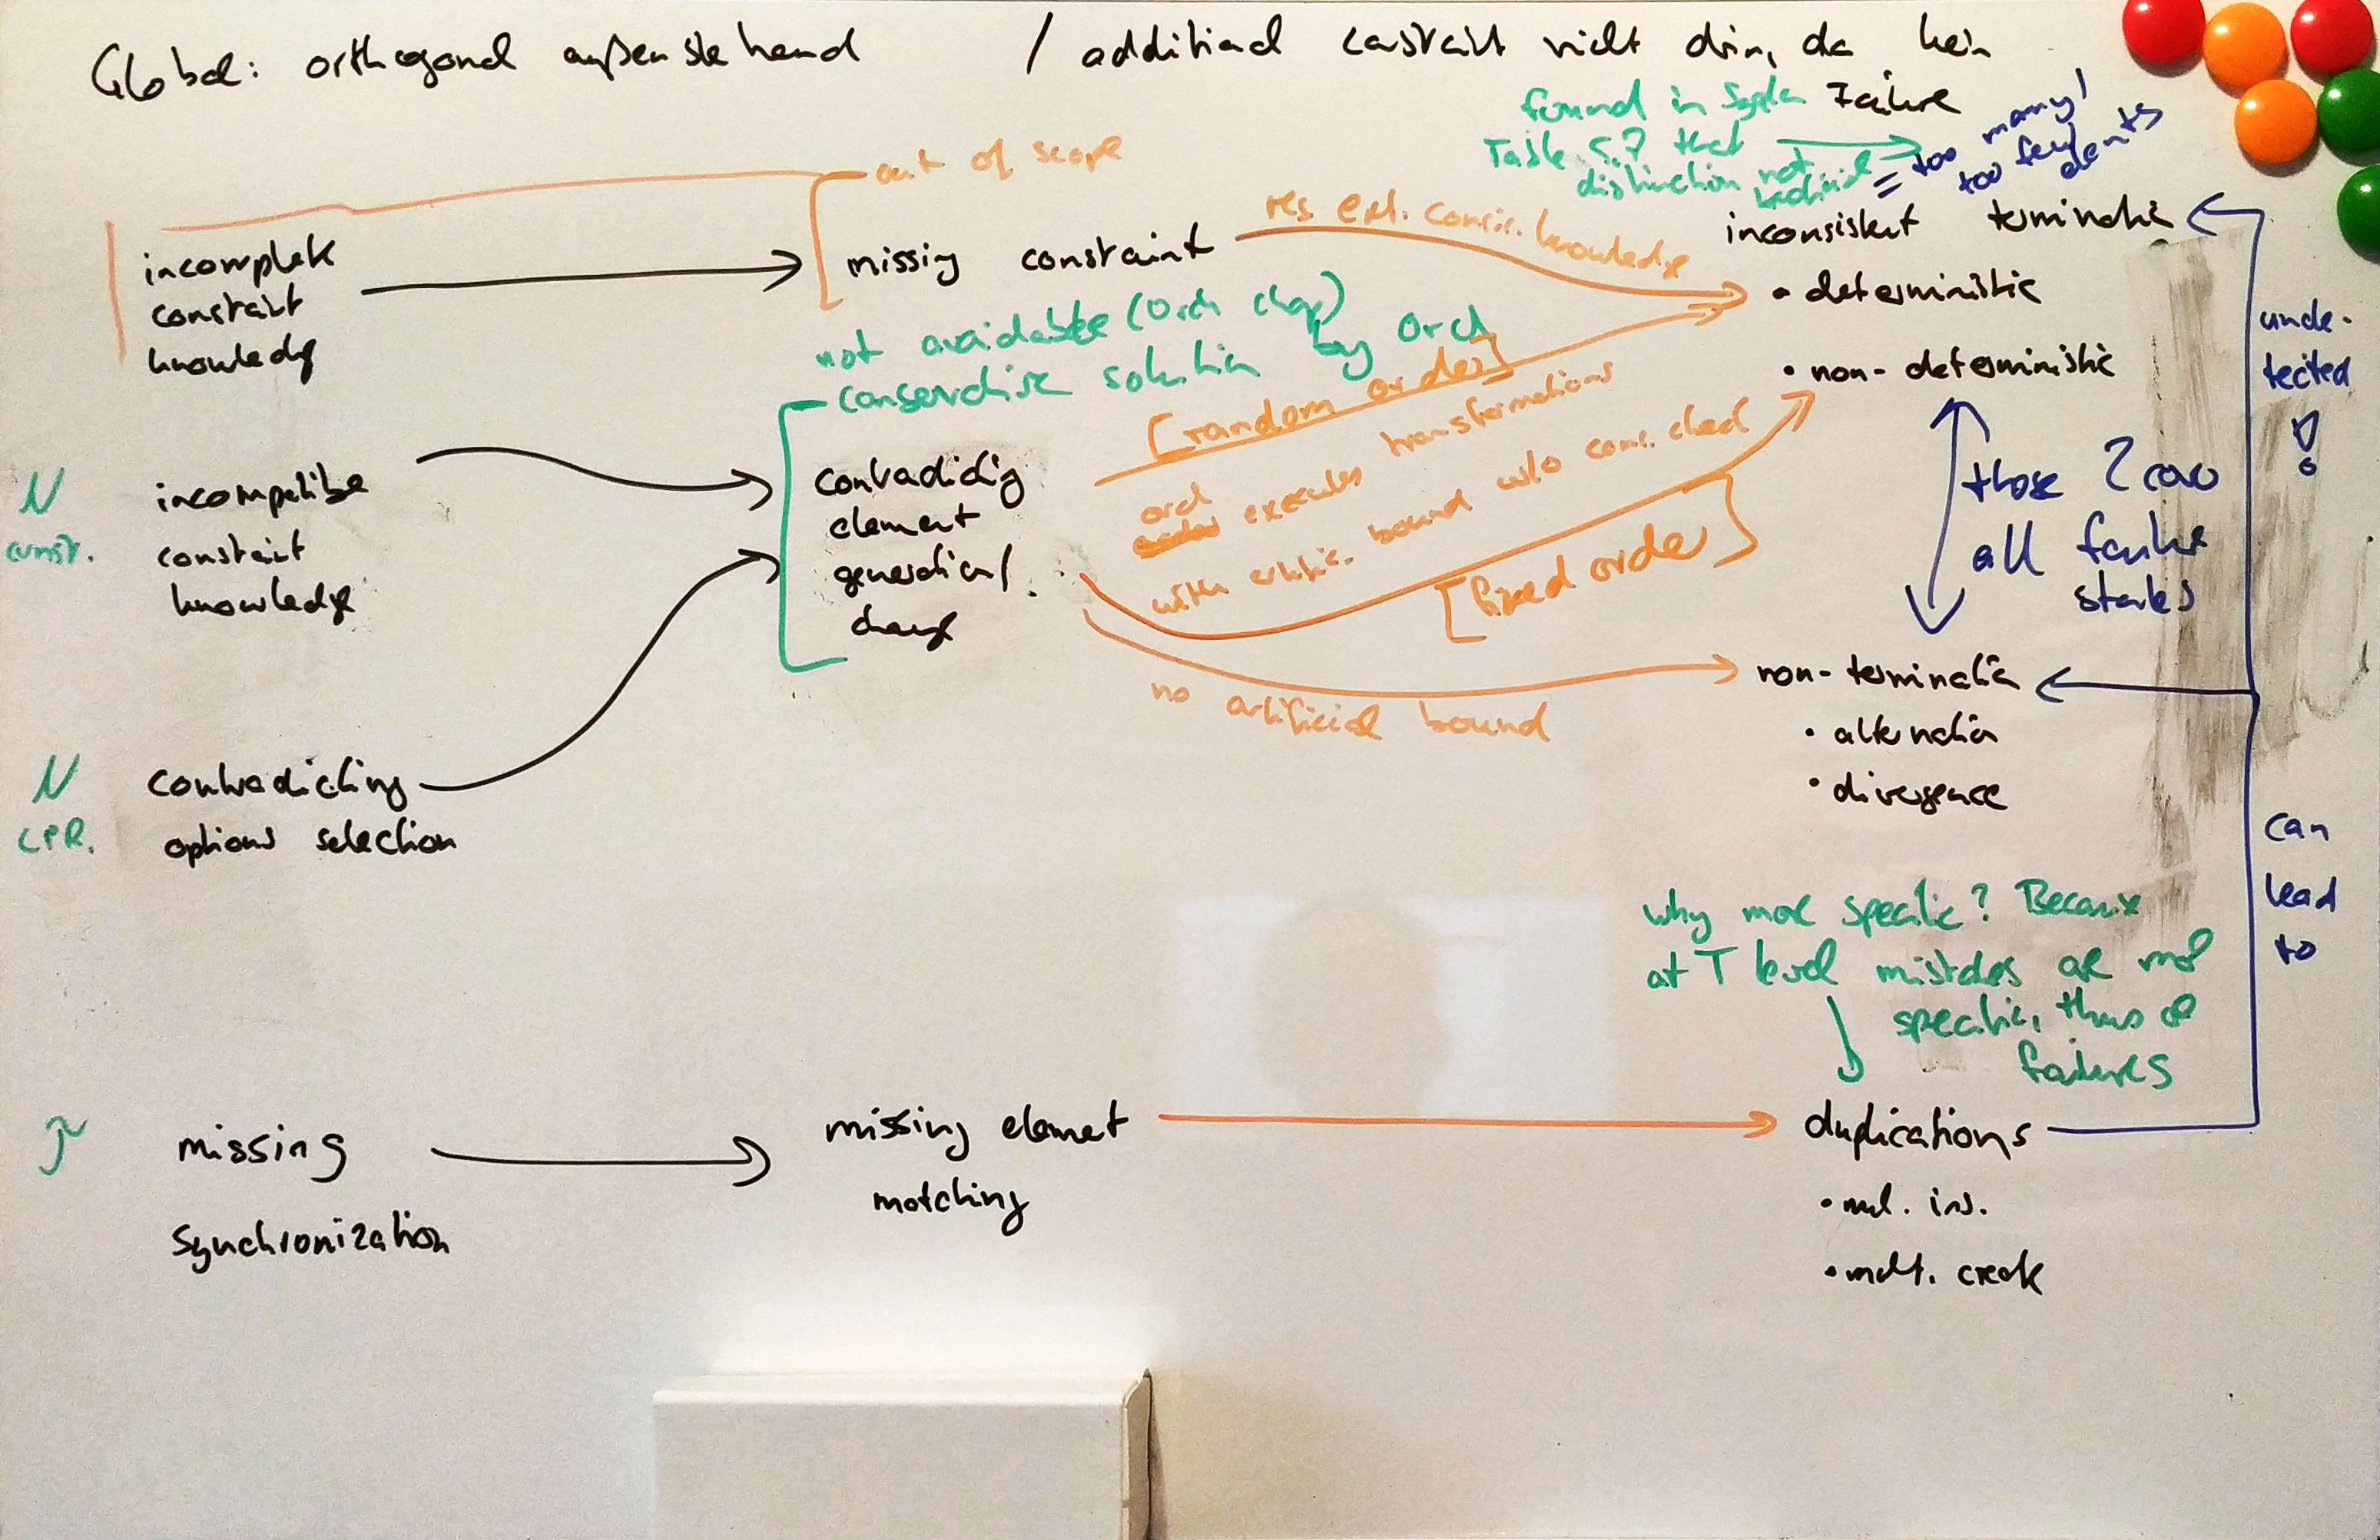
\includegraphics[width=\textwidth]{figures/correctness/errors/categorization.jpg}
    \caption[Categorization of mistakes, faults and failures]{Categorization of mistakes, faults and failures. Adapted from~\owncite[Fig.~3]{klare2019icmt}.}
    \label{fig:errors:categorization}
\end{figure}

\mnote{Failures depending on application algorithm}
In \autoref{fig:errors:categorization}, we depict the different failure types with their specializations, which we discuss in the following.
Note that we do not assume a specific application algorithm when discussing failures.
Whether a potential failure occurs or not highly depends on the used algorithm.
For example, using the provenance algorithm proposed in \autoref{chap:orchestration:algorithm} will neither lead to non-termination nor to inconsistent models, at least if the consistency check is implemented properly, but may only lead to returning $\bot$.
Having an artificial upper bound for the number of transformation executions, of course, always prevents from non-termination.
Only if transformations are executed without checking consistency afterwards or without defining an execution bound, the discussed failures can actually occur.
Whenever an algorithm returns $\bot$, this can, however, be an indicator whether the algorithm fails because an artificial execution bound was reached or because a transformation cannot be applied anymore as it is not able to process the given changes.
We will discuss that in \autoref{chap:errors:avoidance}.

We further distinguish the already discussed failure types as follows.
\begin{properdescription}
    \item[Inconsistent Termination:] %\mnote{Termination in inconsistent states}
    Inconsistent termination means that the application algorithm terminates and the models it returns are inconsistent.
    This can only occur if the algorithm does not check the models, which the application of the transformations yields, for consistency.
    Furthermore it can terminate \emph{deterministically} or \emph{non-deterministically}, depending on whether each execution delivers the same inconsistent models or different ones, because different execution orders of the transformations are selected.

    \item[Non-Termination:] %\mnote{Non-termination in terms of alternation or divergence}
    Non-termination means that the application algorithm does not terminate but executes transformations indefinitely without achieving a consistent state of the models.
    We can further distinguish between \emph{alternation} and \emph{divergence} as defined in \autoref{def:applyalternation}.
    Alternation means that the same model states are produced repeatedly, which can, for example, be because a feature, such as an attribute or reference, alternates between two or more values.
    In other cases, divergence occurs, which means that some feature values are changed indefinitely, such as a number counting up, a string being appended repeatedly, or an infinite number of elements being created.
    While an alternating algorithm can easily run endlessly, a diverging algorithm will abort at some point in time in many cases, because endless element creation or string concatenation can lead to an overflow of available memory.
    
    \item[Returning $\bot$:] %\mnote{Termination without yielding consistent models}
    The application algorithm may terminate and return $\bot$ to indicate that it was not able to find an orchestration that yields consistent models.
    This may either be because no such orchestration exists or can be found even though no mistakes were made, or because the transformation network actually contains faults that prevents the algorithm from finding a consistent orchestration.
    For example, if transformations are not synchronizing, the application algorithm will, in general, not be able to execute them in a way that they deliver consistent models.
    This kind of failure is different from the others, as it is intended behavior of the algorithm to return $\bot$ rather than returning inconsistent models or not terminating at all, but it is still not the intended result as it is caused by an actual fault.

    \item[Duplications:] %\mnote{Element duplications as a special case leading to non-termination or inconsistent termination}
    As a more specific failure case, we have introduced element duplications, which can especially arise if transformations are not synchronizing and thus do not match existing elements rather than creating new ones.
    We can further separate this into \emph{multiple instantiation} and \emph{multiple insertion}. 
    Multiple instantiation can occur because different consistency preservation rules instantiate an element multiple times, although all of them represent the same one.
    Multiple insertion can occur because an element is inserted into a reference or attribute list several times, although it should be inserted only once. 
    In fact, such duplications can ultimately lead to inconsistent termination, non-termination, or returning $\bot$, either because the algorithm returns after a finite number of transformation executions without checking consistency or returning $\bot$, or because the transformations are not able to restore consistency and the algorithm does thus not terminate.
    Duplications, however, represent a special case, which, as we will see in the evaluation in \autoref{chap:correctness_evaluation}, is one of the most important error cases for transformation networks.
    Thus, identifying such duplications in the generated models can ease finding the causal mistake in terms of missing synchronization.
\end{properdescription}

\mnote{Consistency checks problematic}
We have discussed that if an application algorithm checks consistency and has an artificial execution bound, it will only return $\bot$ rather than producing any other type of failure, especially not the more specific duplications. 
Knowing the other failure types and their relation to the causal mistakes is still important.
First, when a transformation network with such an application algorithm yields $\bot$ in most execution scenarios, there will likely be a fault in the transformation implementations.
Temporarily replacing the algorithm with a less restrictive one can help to find the reasons, because then, for example, duplications may be detectable that help to identify missing synchronization.
Second, in many transformation languages consistency relations are not represented explicitly, thus consistency checks are performed by executing the transformation and checking whether changes were performed.
Then, if transformations are non-synchronizing, they return an actually inconsistent state, which may, however, not be identified by the transformation as such.
This is due to the fact that these transformations do not expect to be used in the synchronization scenario and thus assume that consistency is achieved by construction, i.e., that only changes for one model are given and must be processed and, thus, that the models are consistent after executing the consistency preservation rules.


\subsection{Mistake and Fault Types}
\label{chap:errors:categorization:mistakes}

\mnote{Mistakes by specification levels}
Developers can make different kinds of mistakes at each of the specification levels, which lead to faults in the implementation of transformations and eventually to different kinds of failures during transformation execution.
In the following, we derive mistakes and faults from the specification levels, as depicted in \autoref{fig:errors:categorization}.

\mnote{Excluded mistake types}
We explicitly focus on conceptual mistakes and faults concerned with the development of transformation networks.
This especially excludes the following two types of mistakes.
\begin{properdescription}
    \item[Technical Mistakes:] We do not consider technical and careless mistakes that are due to misuse of the transformation language, a coding error such as a missing handling of \emph{null} values, or comparable mistakes.
    \item[Transformation Incorrectness:] We do not consider any kinds of mistakes that lead to incorrect transformations. We assume that transformations are correct, i.e., that the consistency preservation rules produce results that are consistent to their consistency relations. Thus any mistake related to the transformations handling changes in only one of the models are out of scope, as these scenarios are part of research regarding the individual bidirectional transformations on their own. However, mistakes regarding synchronization of transformations, i.e., the case that changes were performed to both models, are relevant.
\end{properdescription}
In fact, technical mistakes eventually lead to incorrectness of the transformations.


\subsubsection*{\LevelTransformation Level}

\mnote{Correctness by synchronizing transformations}
Correctness at the \leveltransformation level requires each transformation to be synchronizing.
We have discussed in \autoref{chap:synchronization:achieving} that the essential requirement to make ordinary transformations synchronizing is the matching of existing elements, because transformations that were not developed for the synchronization case do usually not assume elements to be already existing but to be either added by changes that are processed by the transformation or created by the transformation itself.

\mnote{Missing knowledge about synchronization}
The mistake a transformation developer can make at this level is not to consider that synchronization is necessary, potentially because he or she does not even know that it is necessary. Then the transformation may be correct but not synchronizing.
In the implementation, this manifests as the absence of necessary matchings of elements.
We have already discussed that this finally leads to the duplicate creation or insertion of model elements when executing such transformations.


\subsubsection*{\LevelNetworkRelation Level}

\mnote{Correctness by combination or individual}
The \levelnetworkrelation level concerns correctness of the consistency relations in a transformation network.
In general, we can distinguish two notions of correctness for them, as discussed in \autoref{chap:correctness:notions_correctness}.
First, relations must reflect an intended, probably informal notion of consistency.
If the relations miss to reflect constraints of that notion or if they reflect additional constraints that are not part of that notion, the relations may be considered incorrect.
Second, the relations must be compatible.
As discussed in \autoref{chap:compatibility}, this is necessary to enable the consistency preservation rules to find consistent models at all.
In the worst case, there may not be a single tuple of models that is consistent to all consistency relations when they are incompatible.

\mnote{Individual correctness irrelevant}
The first correctness notion, however, only concerns a single consistency relation rather than the combination of them.
We thus assume it to be correct, as we assume each transformation to already be correct.
Finally, such incorrectness would not even be interesting.
Defining additional constraints does not lead to failures but, in the worst case, only to not finding consistent models although they exist, and missing constraints simply leads to inconsistent models, as the result does not fulfill the constraints of the existing, informal notion of consistency.

\mnote{Correctness requires compatibility}
The relevant correctness notion is the one of compatibility.
One or more transformation developers can make the mistake of having incompatible knowledge about the consistency constraints encoded into the transformations.
This, in consequence, leads to a fault in the implementation of transformations, which may perform a contradicting generation or modification of model elements, for which no orchestration of the transformations may yield consistent models.
Depending on the operation of the application algorithm, this can lead to different types of failures.
If the transformations are executed with an artificial execution bound, the algorithm will terminate with inconsistent models, which may be returned or not depending on whether it checks consistency.
The inconsistency will be deterministic or not, according to whether the execution order of transformations is fixed or not.
If the algorithm does not implement such an artificial bound, such a fault can also lead to non-termination of the algorithm, because the execution of transformations will never lead to consistent models.
Finally, if the algorithm implements an artificial execution bound and consistency checks, it may also return $\bot$ in this case.

\subsubsection*{\LevelNetworkRule Level}

\mnote{No precise correctness notion}
The \levelnetworkrule level concerns correctness of the complete transformations of a network.
We did not give a precise definition of what this correctness means.
In \autoref{chap:orchestration}, we have discussed assumptions to transformations to enable an application function to solve the orchestration problem, which could be a reasonable correctness measure.
We have, however, also discussed that we cannot make any practical assumptions to the transformations such that they improve the ability of the application algorithm to find a consistent orchestration if it exists.

\mnote{Mistake possibility by contradicting options}
We only know from \autoref{chap:orchestration:decidability:restriction} that consistency relations providing multiple options for corresponding elements to consider models consistent can lead to consistency preservation rules that always select elements that are not in the overlap of these options between different transformations.
In consequence, if transformation developers decide to implement consistency preservation rules that make such contradicting selections or generations of elements, the transformations may fail due to the same reasons as discussed for the \levelnetworkrelation level.
In this case, the causing mistake is that the transformation developers make contradicting selections of available options to restore consistency.

\mnote{No complete mistakes overview}
We did not find a property that a transformation set and especially its consistency preservation rules have to fulfill and instead concluded to deal with the orchestration problem by means of a conservative application algorithm.
Thus, we cannot give a reasonable or even complete overview of potential mistakes developers can make at this level.


\subsection{Causal Chains}

\mnote{Mistakes, faults, failures dependencies}
We have already discussed the relevant causal chains between mistakes, faults, and failures when introducing the relevant mistake types.
The full overview of these dependencies is given in \autoref{fig:errors:categorization}.
Mistakes at the \levelnetworkrelation and \levelnetworkrule levels can always lead to any kind of failure, namely non-termination, inconsistent termination, or returning $\bot$, depending on how the application algorithm operates.
Thus, these dependencies do not give any insights regarding which mistakes may have caused an occurring failure.
Mistakes at the \leveltransformation level, however, produce a specific kind of failure that can be distinguished from the general failure types.
Thus, knowing these causal chains is especially useful for identifying mistakes at the \leveltransformation level.
We further discuss the detection and avoidance of mistakes in the subsequent section.

\begin{figure}
    \centering
    \newcommand{\hdistance}{7em}
\newcommand{\classwidth}{6em}

\newcommand{\classdistance}{5em}
\newcommand{\objectwidth}{6.3em}

\begin{tikzpicture}[
    consistency preservation/.style={-latex, consistency changed element, font=\small},
    user change/.style={-latex, user changed element, font=\small},
    legend/.style={font=\footnotesize},
    mininode/.style={inner sep=.25em},
]

% Person
\umlclassvarwidth{person}{}{Person\sameheight}{
firstname\\
lastname
}{\classwidth}

% Employee
\umlclassvarwidth[,above right=1.5em and \hdistance of person.north east, anchor=south]{employee}{}{Employee\sameheight}{
name
}{\classwidth}

\umlclassvarwidth[,below right=1.5em and \hdistance of employee.south, anchor=north west]{resident}{}{Resident\sameheight}{
name
}{\classwidth}


% CONSISTENCY RELATIONS
\draw[consistency relation] (person.north) |- node[pos=0, above left] {$p$} node[pos=0.75, above] {$\consistencyrelation{CR}{PE}$} node[pos=1, above left] {$e$} (employee.west);
\draw[consistency relation] (employee.east) -| node[pos=0, above right] {$e$} node[pos=0.3, above] {$\consistencyrelation{CR}{ER}$ / $\consistencyrelation{CR}{ER}'$} 
node[pos=1, above right] {$r$} (resident.north);
\draw[consistency relation] (resident.west) -- node[pos=0, below left] {$r$} node[pos=0.5, below] {$\consistencyrelation{CR}{PR}$ / $\consistencyrelation{CR}{PR}'$} node[pos=1, below right] {$p$} (resident.west-|person.east);

%\draw[consistency relation 2] (person.east) -- node[pos=0, below right] {$p$} ++(0.35*\hdistance,0) -- node[pos=0, right=0.5em] {$R_{PER}$} node[pos=1, above left] {$e$} ([yshift=1em]employee.south west);
%\draw[consistency relation 2, ->] ([xshift=0.35*\hdistance]person.east) -- node[pos=1, below left] {$r$} ([yshift=-1em]resident.north west);

% \node[consistency related element 2, below left=5em and 2.5em of person.south west, anchor=north west] (relations1) {
% $\begin{aligned}
%     R_{PER} =\; &
%             \setted{\tupled{p,e,r} \mid \\
%             & p.firstname + "\text{\textvisiblespace}" + p.lastname = e.name = r.name\\
%             & \land p.address = r.address%\\
%             %& 
%             \land p.income = e.salary\\
%             & \land e.socsecnumber = r.socsecnumber
%         }
% \end{aligned}$
% };

%\node[consistency related element, below=0.5em of relations1.south west, anchor=north west] {
\node[consistency related element, below left=1.2em and 0em of person.south west, anchor=north west, inner sep=0em] {
$\begin{aligned}
    \consistencyrelation{CR}{PE} =\; &
            \setted{\tupled{p,e} \mid %\\
            %& 
            \mathvariable{p.firstname} + "\text{\textvisiblespace}" + \mathvariable{p.lastname} = \mathvariable{e.name}%\\
            %& \land p.income = e.salary
        }\\[0.3em]
    \consistencyrelation{CR}{PR} =\; &
            \setted{\tupled{p,r} \mid %\\
            %& 
            \mathvariable{p.firstname} + "\text{\textvisiblespace}" + \mathvariable{p.lastname} = \mathvariable{r.name}%\\
            %& \land p.address = r.address
        }\\
    \consistencyrelation{CR}{PR}' =\; &
            \setted{\tupled{p,r} \mid %\\
            %& 
            \mathvariable{p.lastname} + "\text{\textvisiblespace}" + \mathvariable{p.firstname} = \mathvariable{r.name}%\\
            %& \land p.address = r.address
    }\\[0.3em]
    \consistencyrelation{CR}{ER} =\; &
            \setted{\tupled{e,r} \mid %\\
            %& 
            \mathvariable{e.name} = \mathvariable{r.name}%\\
            %& \land e.socsecnumber = r.socsecnumber
        }\\
    \consistencyrelation{CR}{ER}' =\; &
            \setted{\tupled{e,r} \mid %\\
            %& 
            \mathvariable{e.name.toLower} = \mathvariable{r.name}%\\
            %& \land e.socsecnumber = r.socsecnumber
        }
\end{aligned}$
};

% % LEGEND
% \coordinate (legend_anchor) at ([xshift=1.5*\classwidth,yshift=-2.7*\classdistance]employee);

% \node[draw=darkgray, matrix, legend, nodes=mininode, below=0em of legend_anchor, anchor=north, outer sep=0, inner sep=0.4em, column sep=0.2em, row sep=-0.2em] (legend) {
%     \draw[consistency relation] (0,0) -- (1.4em,0); &
%     \node[consistency related element, anchor=west] {consistency constraint}; \\
%     %
%     \draw[-latex, user changed element] (0,0) -- (1.4em,0); &
%     \node[user changed element, anchor=west] {user change}; \\
%     %
%     \draw[-latex, consistency changed element] (0,0) -- (1.4em, 0); &
%     \node[consistency changed element, anchor=west, align=left] (legend_cpr_label) {consistency preservation};\\
% };

\end{tikzpicture}


%    \includegraphics[angle=270, width=\textwidth]{figures/mistakes_examples_employee.pdf}
    \caption[Adaptation of consistency relations from running example]{Adaptation of consistency relations from the extended running example in \autoref{fig:compatibility:three_persons_example_extended}. Adapted from~\owncite[Fig.~5]{klare2019icmt}.}
    \label{fig:errors:mistake_effects_example_metamodels}
\end{figure}

\begin{figure}
    \centering
    \newcommand{\hdistance}{7em}
\newcommand{\classwidth}{6em}

\newcommand{\classdistance}{5em}
\newcommand{\objectwidth}{6.3em}

\begin{tikzpicture}[
    consistency preservation/.style={-latex, consistency changed element, font=\small},
    user change/.style={-latex, user changed element, font=\small},
    legend/.style={font=\footnotesize},
    mininode/.style={inner sep=.25em},
]

% LEVEL 1 ERROR
\coordinate (failure_l1_anchor) at (0,0);
\node[above=0.5em of failure_l1_anchor] {\textbf{\LevelTransformation Level Mistake} ($R_{PE}, R_{PR}, R_{ER}$)};

\umlobjectvarwidth[, fill=white, below=0 of failure_l1_anchor, anchor=north]{l1_employee}{}{
: Employee}{
name="Alice Avid"
}{\objectwidth}

\umlobjectvarwidth[, fill=white, below left=0.4*\classdistance and \classdistance+\classwidth of l1_employee.north, anchor=north] {l1_person}{}{
: Person}{
firstname="Alice"
lastname="Avid"
}{\objectwidth}

\umlobjectvarwidth[, fill=white, above right=1em and 2*\classdistance+2*\classwidth of l1_person.center, anchor=south] {l1_resident}{}{
: Resident}{
name="Alice Avid"
}{\objectwidth}

\umlobjectvarwidth[, fill=white, above right=0.5em and 2*\classdistance+2*\classwidth of l1_person.center, anchor=north] {l1_resident_duplicate}{}{
: Resident}{
name="Alice Avid"
}{\objectwidth}

\umlhuman{l1_human}{at ([xshift=1em, yshift=3em]l1_person.north west)}{user changed element}{}{0.5}
\draw[user change] ([xshift=1em,yshift=1.8em]l1_person.north west) -- node[right, align=center] {1. +} ([xshift=1em]l1_person.north west);
\draw[consistency preservation] ([yshift=1em]l1_person.east) -- node[above] {2. +} ([yshift=0em]l1_employee.west);
\draw[consistency preservation] (l1_employee.east) -- node[above] {3. +} (l1_resident.west);
\draw[consistency preservation] (l1_resident_duplicate.west-|l1_person.east) -- node[below] {4. +} (l1_resident_duplicate.west);


% LEVEL 2 ERROR
\coordinate (failure_l2_anchor) at ([yshift=-1.8*\classdistance]failure_l1_anchor);
\node[above=0.5em of failure_l2_anchor] {\textbf{\LevelNetworkRelation Level Mistake} ($R_{PE}, R_{PR}, R_{ER}'$)};

\umlobjectvarwidth[, fill=white, below=0 of failure_l2_anchor, anchor=north]{l2_employee}{}{
: Employee}{
name="Alice Avid"
}{\objectwidth}

\umlobjectvarwidth[, fill=white, below=0.7*\classdistance of l2_employee.north, anchor=north]{l2_employee2}{}{
: Employee}{
name="alice avid"
}{\objectwidth}

\umlobjectvarwidth[, fill=white, below left=0.4*\classdistance and \classdistance+\classwidth of l2_employee.north, anchor=north] {l2_person}{}{
: Person}{
firstname="Alice"
lastname="Avid"
}{\objectwidth}

\umlobjectvarwidth[, fill=white, below=0.9*\classdistance of l2_person.north, anchor=north]{l2_person2}{}{
: Person}{
firstname="alice"
lastname="avid"
}{\objectwidth}

\umlobjectvarwidth[, fill=white, right=2*\classdistance+2*\classwidth of l2_person.center, anchor=center] {l2_resident}{}{
: Resident}{
name="alice avid"
}{\objectwidth}

\umlhuman{l2_human}{at ([xshift=1em, yshift=3em]l2_person.north west)}{user changed element}{}{0.5}
\draw[user change] ([xshift=1em,yshift=1.8em]l2_person.north west) -- node[right, align=center] {1. +} ([xshift=1em]l2_person.north west);
\draw[consistency preservation] ([yshift=1em]l2_person.east) -- node[above] {2. +} ([yshift=0em]l2_employee.west);
\draw[consistency preservation] (l2_employee.east) -- node[above] {3. +} ([yshift=1em]l2_resident.west);
\draw[consistency preservation] ([yshift=0em]l2_resident.south) |- node[pos=0.75, above] {4. +} (l2_person2.east);
\draw[consistency preservation] ([yshift=1em]l2_person2.east) -- node[above] {5. +} ([yshift=-0.5em]l2_employee2.west);


% LEVEL 3 ERROR
\coordinate (failure_l3_anchor) at ([yshift=-2.6*\classdistance]failure_l2_anchor);
\node[above=0.5em of failure_l3_anchor] {\textbf{\LevelNetworkRule Level Mistake} ($R_{PE}, R_{PR}', R_{ER}$)};

\umlobjectvarwidth[, fill=white, below=0 of failure_l3_anchor, anchor=north]{l3_employee}{}{
: Employee}{
name="Alice Avid"
}{\objectwidth}

\umlobjectvarwidth[, fill=white, below=1.7*\classdistance of l3_employee.north, anchor=north]{l3_employee2}{}{
: Employee}{
name="Avid Alice"
}{\objectwidth}

\umlobjectvarwidth[, fill=white, below left=0.5*\classdistance and \classdistance+\classwidth of l3_employee.north, anchor=north] {l3_person}{}{
: Person}{
firstname="Alice"
lastname="Avid"
}{\objectwidth}

\umlobjectvarwidth[, fill=white, below=0.9*\classdistance of l3_person.north, anchor=north]{l3_person2}{}{
: Person}{
firstname="Avid"
lastname="Alice"
}{\objectwidth}

\umlobjectvarwidth[, fill=white, right=2*\classdistance+2*\classwidth of l3_person.center, anchor=center] {l3_resident}{}{
: Resident}{
name="Alice Avid"
}{\objectwidth}

\umlobjectvarwidth[, fill=white, below=0.7*\classdistance of l3_resident.north, anchor=north]{l3_resident2}{}{
: Resident}{
name="Avid Alice"
}{\objectwidth}

\umlhuman{l3_human}{at ([xshift=1em, yshift=3em]l3_person.north west)}{user changed element}{}{0.5}
\draw[user change] ([xshift=1em,yshift=1.8em]l3_person.north west) -- node[right, align=center] {1. +} ([xshift=1em]l3_person.north west);
\draw[consistency preservation] ([yshift=1.5em]l3_person.east) -- node[above] {2. +} ([yshift=0em]l3_employee.west);
\draw[consistency preservation] ([yshift=0em]l3_employee.east) -- node[above] {3. +} ([yshift=1em]l3_resident.west);
\draw[consistency preservation] ([yshift=-0em]l3_resident.west) -- node[above] {4. -} ([yshift=0em]l3_person.east);
\draw[consistency preservation] ([yshift=-0.5em]l3_resident.west) -- node[above] {4. +} ([yshift=1em]l3_person2.east);
\draw[consistency preservation] ([yshift=-1em]l3_person2.east) -- node[above] {5. +} ([yshift=0.5em]l3_employee2.west);
\draw[consistency preservation] ([yshift=1em]l3_person.east) -- node[below] {5. -} ([yshift=-0.5em]l3_employee.west);
\draw[consistency preservation] ([yshift=0.5em]l3_employee2.east) -- node[above] {6. +} ([yshift=-0.5em]l3_resident2.west);
\draw[consistency preservation] ([yshift=-0.5em]l3_employee.east) -- node[below] {6. -} ([yshift=0.5em]l3_resident.west);
\draw[consistency preservation] ([yshift=-1em]l3_resident.west) -- node[below] {7. -} ([yshift=0.5em]l3_person2.east);
\draw[consistency preservation] (l3_resident2.south) |- ++(-5.3*\classdistance, -0.6*\classdistance) node[pos=0.85, above] {7. +} |- (l3_person.west);

% LEGEND
%\coordinate (legend_anchor) at ([xshift=1.5*\classwidth,yshift=-2.7*\classdistance]employee);
\coordinate[below=0.4*\classdistance of l3_employee2.south] (legend_anchor);

\node[draw=darkgray, matrix, legend, nodes=mininode, below=0em of legend_anchor, anchor=north, outer sep=0, inner sep=0.4em, column sep=0.2em, row sep=-0.2em] (legend) {
    %\draw[consistency relation] (0,0) -- (1.4em,0); &
    %\node[consistency related element, anchor=west] {consistency constraint}; \\
    %
    \draw[-latex, user changed element] (0,0) -- (1.4em,0); &
    \node[user changed element, anchor=west] {user change}; & 
    %
    \node {}; &
    %
    \draw[-latex, consistency changed element] (0,0) -- (1.4em, 0); &
    \node[consistency changed element, anchor=west, align=left] (legend_cpr_label) {transformation};\\
};


\end{tikzpicture}


%    \includegraphics[angle=270, width=\textwidth]{figures/mistakes_examples_employee.pdf}
    \caption[Examples for mistakes at different knowledge levels]{Examples for transformation executions based on the consistency relations given in \autoref{fig:errors:mistake_effects_example_metamodels} with mistakes at each of the three specification levels. Arrows denote user changes and transformation executions with numbers indicating their order and +/- indicating element addition and removal. Adapted from~\owncite[Fig.~5]{klare2019icmt}.}
    \label{fig:errors:mistake_effects_example_cases}
\end{figure}

\mnote{Mistake examples at each level}
In \autoref{fig:errors:mistake_effects_example_metamodels}, we depict slightly modified consistency relations from the running example.
Based on these consistency relations, \autoref{fig:errors:mistake_effects_example_cases} depicts three scenarios of transformation executions with mistakes at each of the three introduced levels.
Each scenario assumes a person to be introduced by a user change.
Then transformations are executed and produce changes in the order depicted by the numbers at the transformation executions.
The creation and deletion of an element is denoted by a \enquote{+} and \enquote{-}, respectively.
In one transformation step, multiple elements may be created or deleted.
The arrows indicate that the change of the source element leads to the creation or deletion of the target element.

\mnote{Missing synchronization}
The example for the \leveltransformation level considers the compatible consistency relations $\consistencyrelation{CR}{PE}$, $\consistencyrelation{CR}{PR}$, and $\consistencyrelation{CR}{ER}$. It assumes that the transformation developer made the mistake of not considering the necessity of synchronization, thus not implementing a matching of existing elements.
This can lead to the depicted failure that two residents with the same $\mathvariable{name}$ may be created by both the transformation between employees and residents, as well as the one between persons and residents.
In consequence, the transformations may not be able to process the occurring situation, or, as discussed before, assume consistency by construction and thus identify the models as consistent although they are not.

\mnote{Incompatibility}
The example for the \levelnetworkrelation level considers the incompatible consistency relations $\consistencyrelation{CR}{PE}$, $\consistencyrelation{CR}{PR}$, and $\consistencyrelation{CR}{ER}'$. Thus, the transformation developers made the mistake of not having a compatible knowledge about consistency constraints.
In consequence, the developed transformations may try to resolve the occurring inconsistencies by adding further elements required to fulfill the consistency relations.
This results in the depicted models, which are not consistent to $\consistencyrelation{CR}{ER}'$, because both employees correspond to the resident without the possibility to add a further resident to which one of the employees corresponds.
In fact, the transformations would need to remove the initially added person and the first employee to restore consistency.
Due to incompatibility, there is no consistent tuple of models containing the initially added person.
The algorithm may fail at the depicted state because the transformation between employees and residents is not able to restore consistency.

\mnote{Contradicting option selection}
Finally, the example for the \levelnetworkrule level considers the consistency relations $\consistencyrelation{CR}{PE}$, $\consistencyrelation{CR}{PR}'$, and $\consistencyrelation{CR}{ER}$.
The relations require that for each person, employee, and resident, one with swapped $\mathvariable{firstname}$ and $\mathvariable{lastname}$ exists.
Whether or not these are reasonable relations, they can be fulfilled by simply adding the appropriate elements.
If, however, the transformation developer decides to resolve an inconsistency after adding an element to one model by adding the corresponding one to the other model and removing other elements in the other model for which no corresponding element exists, this leads to the repeated insertion of persons, employees, and residents with $\mathvariable{firstname}$ and $\mathvariable{lastname}$ concatenated in one order and the removal of them with the inverse concatenation, as depicted in \autoref{fig:errors:mistake_effects_example_cases}.
In fact, the depicted process would proceed after Step 7 from the beginning endlessly, unless the application algorithm stops after a fixed number of transformation executions.
In this case, although transformations were developed synchronizing and relations are compatible, finding consistent models after a change fails, because the transformations are not properly aligned with each other.
This is analogous to the example depicted in \autoref{fig:orchestration:no_orchestration}, for which no orchestration exists.
In fact, this is also a problem of selecting incompatible options, as discussed in \autoref{chap:orchestration:decidability:restriction}, because each transformation always restores consistency in a way that is not consistent with the other transformations, thus selecting an option from the consistency relations that is not in the overlap with consistency relations of the other transformations.

\mnote{Distinguishing network level mistakes}
Whether incompatible constraints or a contradicting selection of options to restore consistency leads to a fault and thus potential failures during execution can often not be distinguished.
This is especially the case when consistency relations are not explicitly defined but assumed to be implied by the image of the consistency preservation rules.
If then the execution of transformations fails because the consistency relations induced by the consistency preservation rules are incompatible, it is unclear whether the, only implicitly known, consistency relations according to which the transformation developer defined the transformations are actually incompatible, or whether the defined transformations only make a contradicting selection of options for restoring consistency, which then implies such incompatible consistency relations.
This is due to the reason that even if a transformation developer knows about different options in the consistency relations, he or she can only express one of them in the consistency preservation rules.
Thus, the consistency relations implied by consistency preservation rules can always only be a subset of the originally intended consistency relations.
For example, when the developers know that two options for name mappings are actually valid and for two transformations they select different of these options, then the consistency relations implied by the implemented consistency preservation rules are actually incompatible, because they contain incompatible name mappings, although in the original knowledge the consistency relations contained both these options, but the consistency preservation rules can only reflect one of them.

